\documentclass[]{article}
\usepackage[T1]{fontenc} 	% codifica dei font
\usepackage[utf8]{inputenc} % lettere accentate da tastiera
\usepackage[italian]{babel} % lingua del documento
\usepackage{url} 			% per scrivere gli indirizzi Internet
\usepackage{graphicx}		% per immagini
\usepackage{afterpage}

\begin{document}
\renewcommand\refname{References \& Documents}
\author{Paolo Roncaglioni \and Stefano Sanitate}
\title{\textbf{Progetto Ingegneria Informatica \\ Documento di Specifica}}
\date{\parbox{\linewidth}{\centering%
  \today\endgraf\bigskip\endgraf\bigskip
  \textbf{Supervisors}\endgraf\bigskip
  Maristella Matera \hspace*{1cm} Vittorio Zaccaria \hspace*{1cm} Florian Daniel}}
\maketitle
\newpage

\begin{abstract}
Questo documento di specifica descrive il culmine delle ricerche riguardo la tecnologia dei ChatBot e dei framework ad essi dedicati. Raccolte quindi informazioni su servizi disponibili e stato dell'arte abbiamo deciso di concretizzare la ricerca in una demo di un Bot che risponde alle esigenze di uno studente del Politecnico di Milano. Dopo una prima parte in cui viene descritto il funzionamento generale del Bot che abbiamo pensato di progettare, si passa ai dettagli e criteri dei test che abbiamo eseguito per poter fare un deployment di una prima semplice demo del progetto descritto. La \textbf{pagina successiva} é una rappresentazione grafica di \textit{cosa} per noi é un chatBot, formalizzando i concetti raccolti e formulati per l'intero corso dello sviluppo del progetto.  
\end{abstract}

\tableofcontents	

\afterpage{%
\thispagestyle{empty}
\begin{figure}
\vspace*{-3cm} 
\hspace*{-1cm}
\centering
\includegraphics[width=2\textwidth, angle =90 ]{botofficial}
\end{figure}
\clearpage
}
\newpage

\section{Generalitá}
Il progetto é ovviamente iniziato con la delineazione dello scopo del bot, cioé che funzionalitá avrebbe dovuto soddisfare e il tipo di utenti che potrebbero servirsene. In un primo momento son venute fuori idee interessanti, ma magari giá presenti (e.g.\ bot orari Trenitalia) e difficilmente migliorabili.
Dopo aver quindi analizzato varie possibilitá di scelta delle funzionalitá del bot, abbiamo infine pensato di progettarne uno a tema Politecnico, che racchiuda un insieme di semplici tool allo studente (o al professore) nella gestione della propria vita universitaria. 

\subsection{Scopo}
La definizione delle caratteristiche funzionali inizia col dividerle in utenti che effettuano la propria registrazione con la coppia <Codice persona, Password> e in utenti che non lo fanno. La registrazione non é ovviamente obbligatoria, ma gli utenti loggati avranno a disposizione piú interazioni personalizzate col bot, oltre che avere tutte quelle possibili per gli utenti normali non loggati.

\paragraph{Logged Users}
\begin{enumerate}
\item \textit{Orario universitario}: richiesta orario delle lezioni, previo inserimento di tutti quei parametri che servono per identificare il corso (nome, corso di studio, sede).
\item \textit{Aule libere}: richiesta elenco aule libere, previa scelta del giorno e orario.
\item \textit{Orario aula}: richiesta elenco corsi e orari di una specifica aula (utile per controllare velocemente se l'aula davanti a te é libera).
\item \textit{Posizione aula}: restituisce semplicemente l'edificio in cui é l'aula (utile per le matricole).
\item \textit{Calendario accademico}: richiesta orario accademico, manda il pdf presente sul sito del Politecnico.
\end{enumerate}

\paragraph{UnLogged Users}
\begin{enumerate}
\item \textit{Orario universitario personalizzato}: stessa cosa della funzionalitá parte utente loggato, ma con i dati a disposizione é possibile avere maggiore accuratezza e non é richiesto l'inserimento dei dati.
\item \textit{Esami}: richiesta elenco degli esami a cui ci si é iscritti.
\item \textit{Informazione esami}: informazioni su esami a cui si é iscritti (i.e.\ aula, orario).
\item \textit{Carriera didattica}: restituzione informazioni generali della propria carriera (e.g.\ media, crediti).
\item \textit{Avvisi generici}: possibilitá di settare avvisi generici con qualsiasi evento di trigger (inizialmente pensata solo uscita voti esami con relativa votazione).
\end{enumerate}

\subsection{Personalitá}
Non sapremmo bene come prendere questa parte, poiché non ci é stato detto nulla in merito. Inizialmente di pensava di supporre che il nostro bot possa rispondere a un set di comandi predefiniti e dati da noi, non lasciando spazio all’utente per eventuali frasi complesse da interpretare. Questo approccio ci avrebbe permesso di tralasciare quasi completamente la parte sul parsing e riconoscimento degli intenti. Man mano che cominciavamo a sviluppare il nostro progetto peró ci é sembrato limitante questo approccio, poiché la vera natura del nostro progetto era di "esplorazione" di questo nuovo ambiente. Abbiamo quindi convenuto che la parte interessante sarebbe stata appunto confrontare le varie soluzioni giá presenti di NLU (natural language understanding) e rendere la conversazione col bot il piú vicino possibile a quella con un umano. Ecco quindi che si delinea l'importanza dell'utilizzo di un FrameWork che abbia queste possibilitá.

\section{Requisiti non funzionali}
Sotto questa voce vanno i requisiti e caratteristiche che impongono vincoli  allo sviluppo del bot, sotto diversi punti di vista. Per ogni problema si cercherá quindi una possibile soluzione di implementazione, che non andremo a sviluppare nella demo in quanto non riteniamo necessario in questo progetto approfondire ulteriormente.

\subsection{Prestazioni \and Price strategies}
Secondo il modello posto sopra, un bot in generale si puó rappresentare con due parti distinte, poste totalmente o in parte su un server esterno. La scelta del server influenzerá sicuramente il numero di interrogazioni che si possono fare, la velocitá di risposta e l'usabilitá in generale, a discapito del prezzo che la piattaforma di hosting ci fará pagare per avere questi servigi. Se si utilizza una soluzione "locale" in cui il proprio pc viene utilizzato come server si avranno sicuramente degli svantaggi rispetto a una soluzione cloud, ma il prezzo sará nullo e le limitazioni (se non date da hardware) non esisterebbero. Ad ora, esplorando le varie possibili scelte, per la fase di testing della demo é stato possibile sempre usufruire delle opzioni "free" della piattaforma di turno. Questo include sia UX che Hosting Server. Inoltre, rientra in questa sezione anche la possibilitá di ridurre query rindondanti attraverso l'implementazione di un minimo di \textit{caching}. Non é una parte da sottovalutare in quanto potrebbe risparmiarci un parte consistente di interrogazioni inutili al sistema e migliorare l'efficienza generale. Si pensava quindi di usare inizialmente un'unico file Json, che viene "guardato" dal codice ogni volta che giunge una nuova interrogazione, e aggiornato se i dati richiesti non sono presenti o troppo vecchi per essere attendibili. É un'implementazione semplice di caching, ma per iniziare puó funzionare.  

\subsection{Privacy e persistenza}
Oltre alle informazioni pubbliche dell'utente, dobbiamo per forza aver a che fare con dati personali (e.g.\ password, codice persona ...) e riservati, che nè gli sviluppatori nè soggetti esterno dovrebbe essere in grado di leggere. Queste informazioni doverebbero, se non vogliamo che l'utente debba sempre inserire le sue credenziali, essere tenute in qualche database esterno criptato in modo che neanche noi possano accedere al contenuto se non per interrogazione da parte del codice. Purtroppo questa problematica é una parte troppo grossa da risolvere in un progetto del genere, e potrebbe tranquillamente portarci via tutto il tempo che abbiamo pensato di dedicare al bot. Non analizzeremo dunque piú a fondo questa sezione. 

\subsection{Scraping}
\begin{quote} 
"Il web scraping (detto anche web harvesting o web data extraction) è una tecnica informatica di estrazione di dati da un sito web per mezzo di programmi software"
\end{quote}
Esso quindi é la parte che si occupa di cercare e raccogliere dati sul web, riordinarli e restituirli al richiedente. Il nostro progetto é strettamente correlato alle informazioni esterne che dobbiamo cercare all'interno (nel nostro caso) del sito del politecnico/beep, che purtroppo non é fornita di comode API che possiamo chiamare nel codice. Viene quindi visto indispensabile un cosiddetto \textit{motore di scraping}, ovvero la parte di codice o software preposto alla raccolta dei dati a noi utili. Anch'esso é un argomento molto (forse troppo) vasto per parlarne in queste poche righe, e purtroppo ci siamo visti costretti a non implementarlo nella prima demo del bot. Al suo posto abbiamo pensato di utilizzare un motore "fake" costruito su un foglio di testo, ma di questo se ne parlerá nella sezione dedicata allo sviluppo della demo. Abbiamo ovviamente fatto ricerche, seppur quasi superficiali, su questo argomento. É venuto fuori che esistono decine e decine soluzioni (free o a pagamento) che offrono web scraping di varia profonditá, integrazioni con API e servizi. Uno in particolare ha attirato la nostra attenzione: un portale free che offre soluzioni di scraping \textit{in teoria facile da programmare} che risponde al nome di \textbf{Portia}. Qualche prova é stata fatta giusto per vedere che cosa si poteva e per adattare al meglio la nostra demo, in una previsione di implementazione futura. Si é concluso che il Json é sempre il mezzo piú semplice e veloce per simulare questi motori.

\section{Flow}
Vengono sotto proposti due tipi differenti di rappresentazioni grafiche, che nel loro insieme dovrebbero comporre la parte dedicata alla UX. La prima infatti, molto simile a un diagramma a flusso, mette ordine sul percorso che la conversazione deve avere, presentando il tipo di risposte che l'utente si deve aspettare dopo determinate interrogazioni (é comunque presente una legenda per aiutare la comprensione). Il secondo, a nostro avviso piú interessante, é simile a un diagramma delle classi, e cerca di mettere in chiaro le relazioni e le caratteristiche degli argomenti della conversazioni (chiamati \textbf{contesti}). Proprio quest'ultimo, essendo piú elaborato, ha bisogno di essere spiegato con una legenda (sotto) e attraverso alcune semplici regole:

\begin{itemize}
\item Una conversazione all'interno di un context puó cominciare da qualsiasi root intent dello stesso context.
\item Il passaggio tra due context può avvenire in qualsiasi momento: a seconda dell'intento che ne permette il passaggio, i parametri vengono tenuti o meno. 
\item Non possono esistere più root intent con le stesse frasi di trigger, possono invece esistere degli intent normali con le stesse frasi.
\item Gli intent tra gli asterischi sono quelli che possono essere usati per le risposte di relazione simmetrica (riconosciute che partono dallo stesso context). Un intent padre passa questa proprietá ai figli.
\item La relazione padre/figlio esiste quando un intento padre contiene nell'imput piú parametri. Per la scelta dell'intent in questa relazione si va a prendere il figlio che necessita di meno parametri per essere "attivato" (seguendo la gerarchia grafica).
\item La relazione tra i context é SERIALE, RIFLESSIVA (tranne poche eccezioni) e SIMMETRICA.
\end{itemize}



\begin{center}
\vspace*{0.05cm}
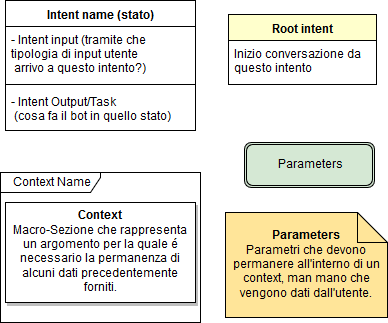
\includegraphics[width=0.6\textwidth]{flow2legend}
\end{center}

\pagebreak
\vspace*{-3cm} 
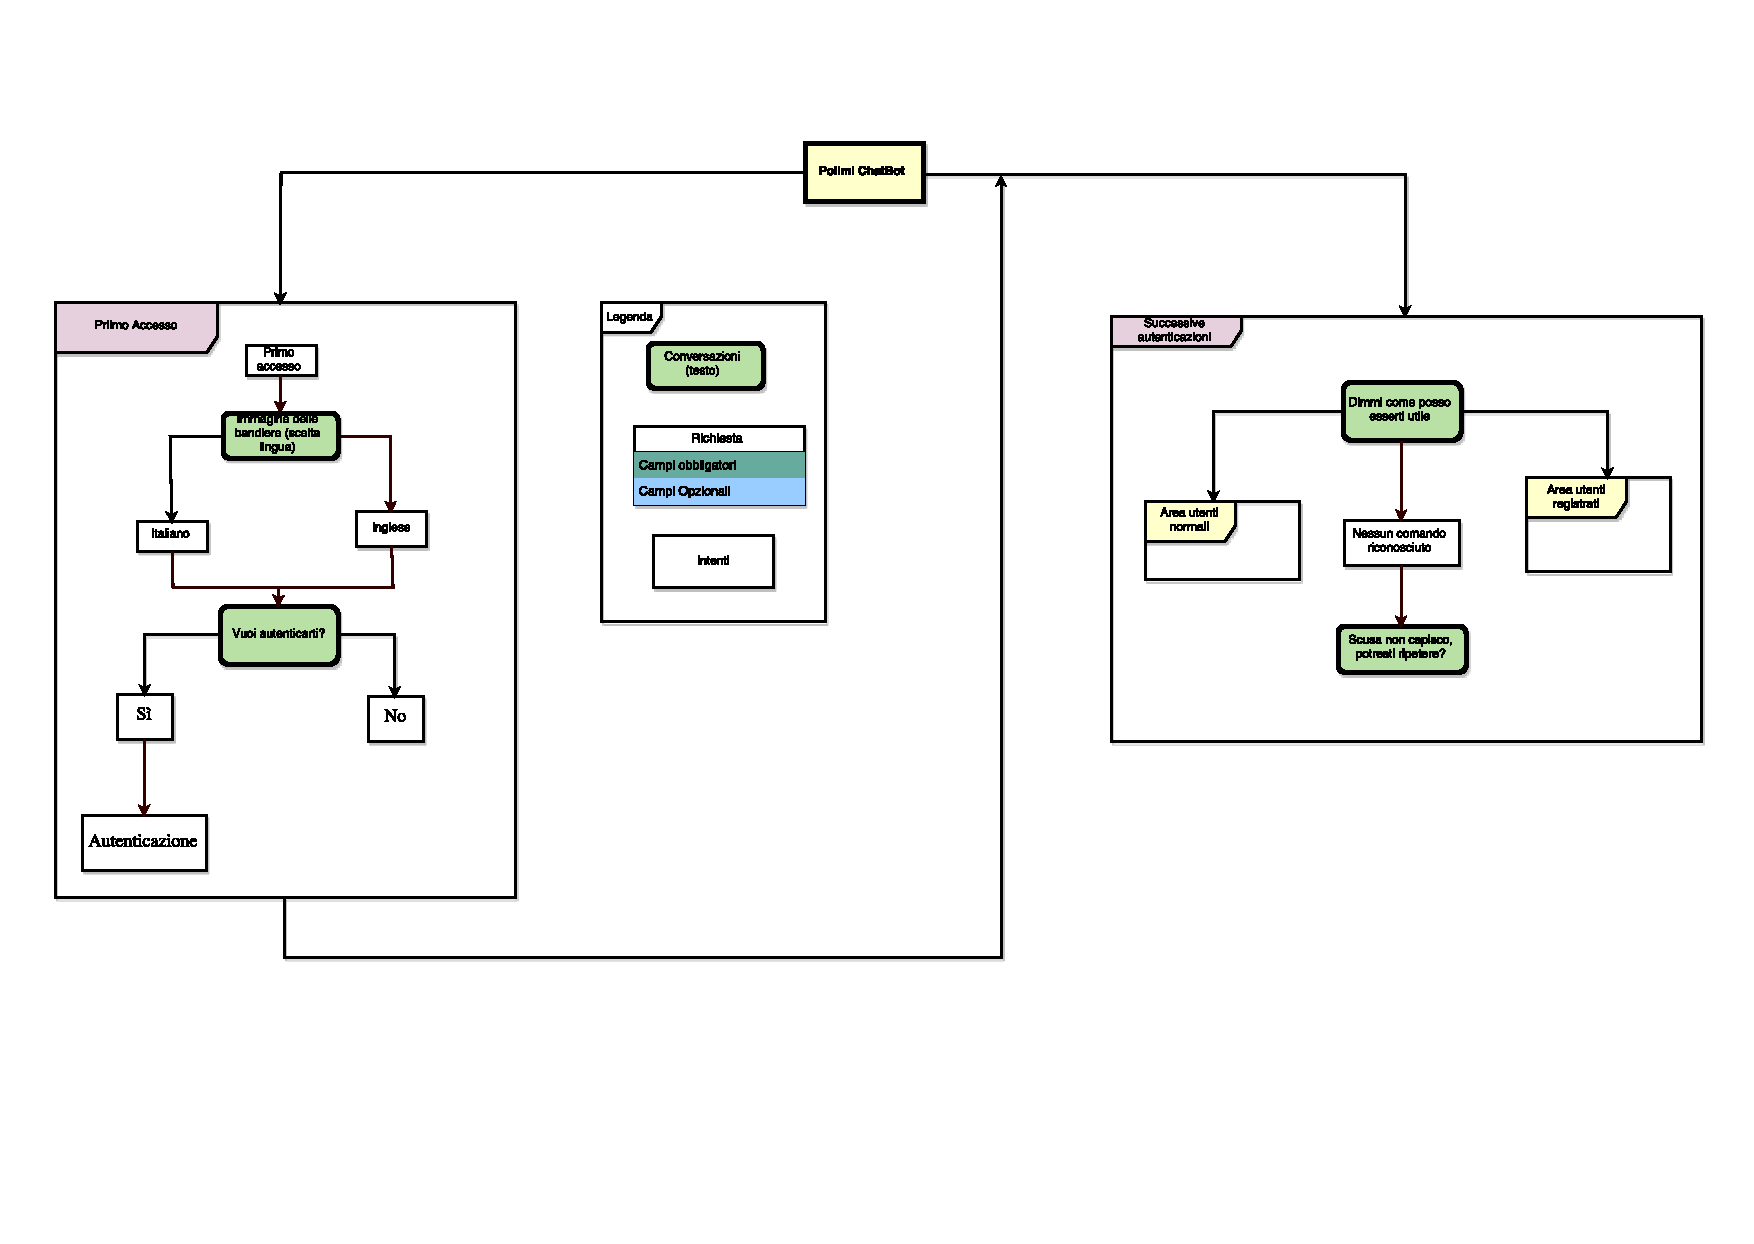
\includegraphics[width=2\textwidth, angle =90 ]{p01}
\thispagestyle{empty}


\vspace*{-3cm}
\hspace*{-2cm} 
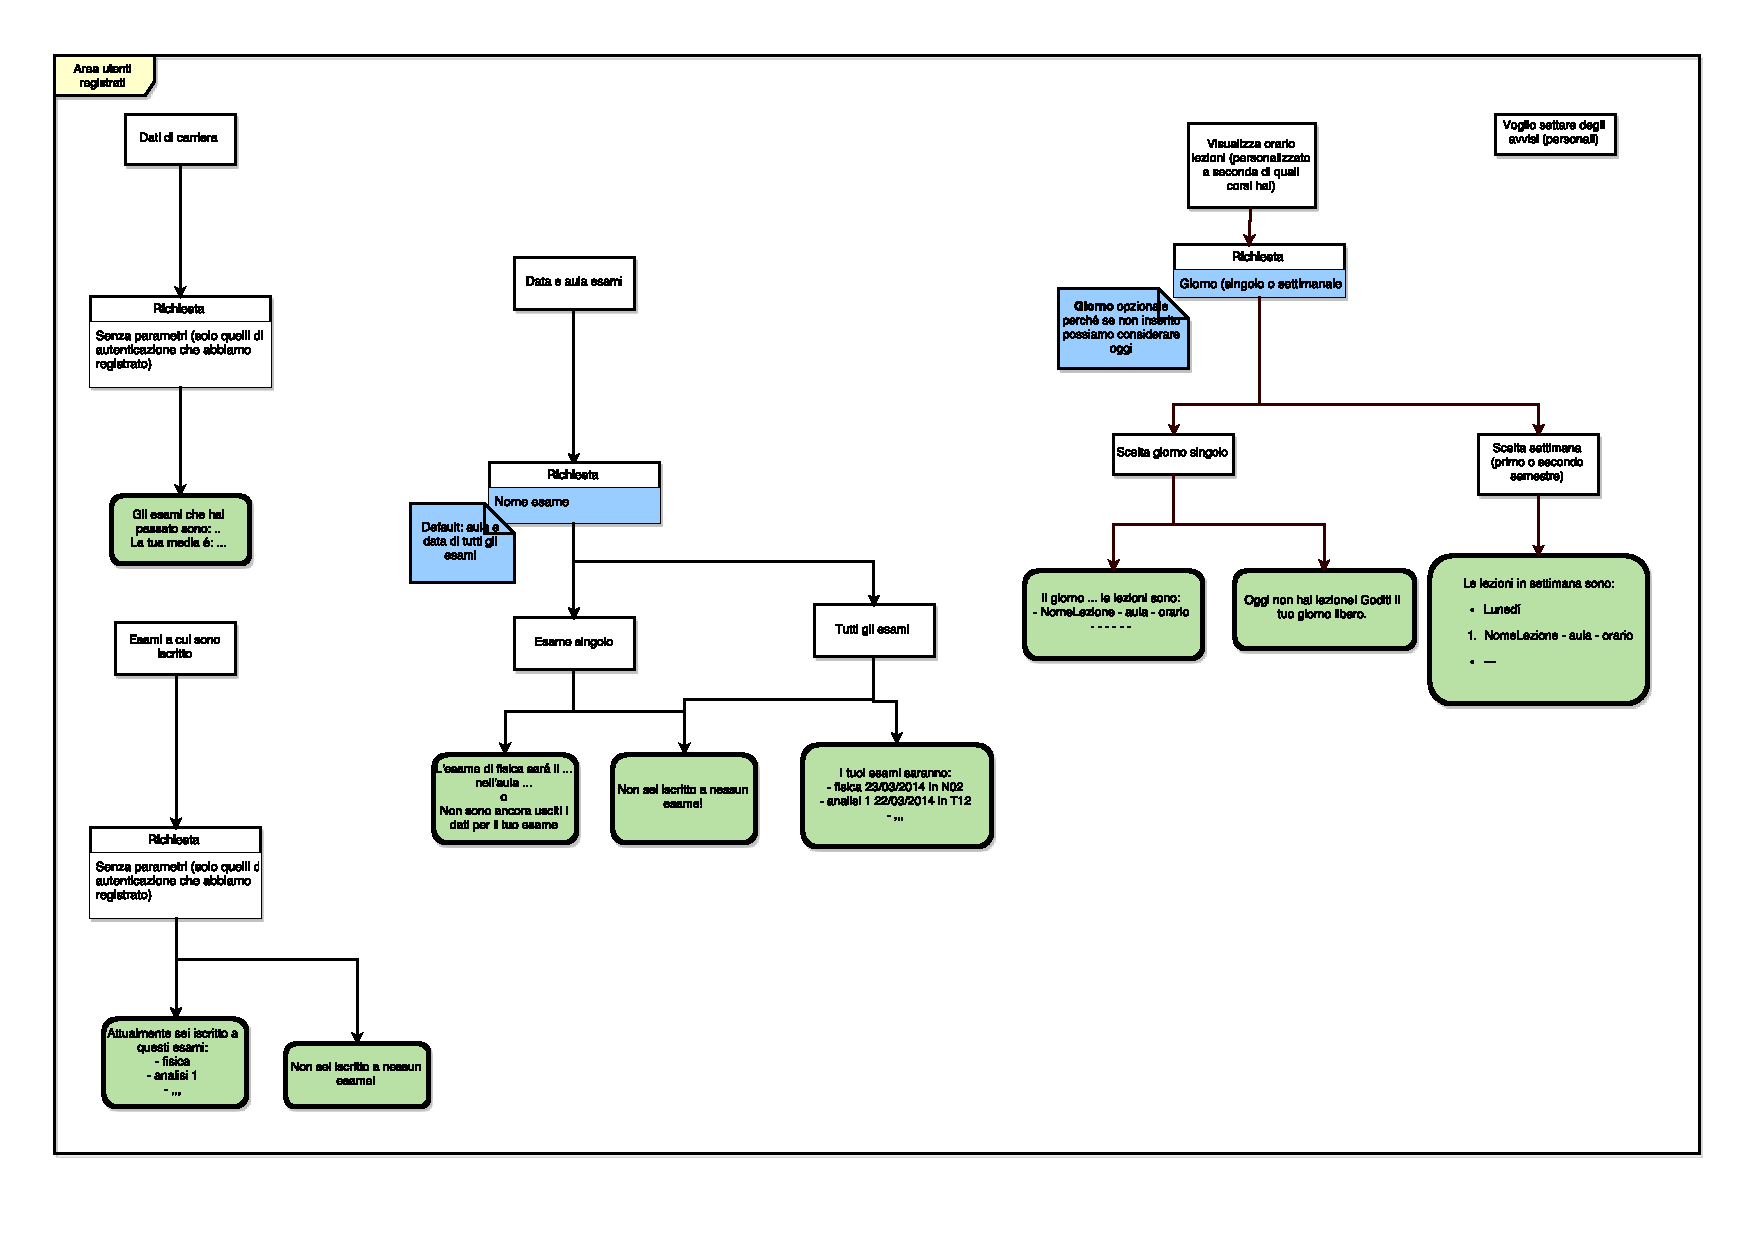
\includegraphics[width=2\textwidth, angle =90 ]{p02}
\thispagestyle{empty}


\vspace*{-3cm}
\hspace*{-2cm} 
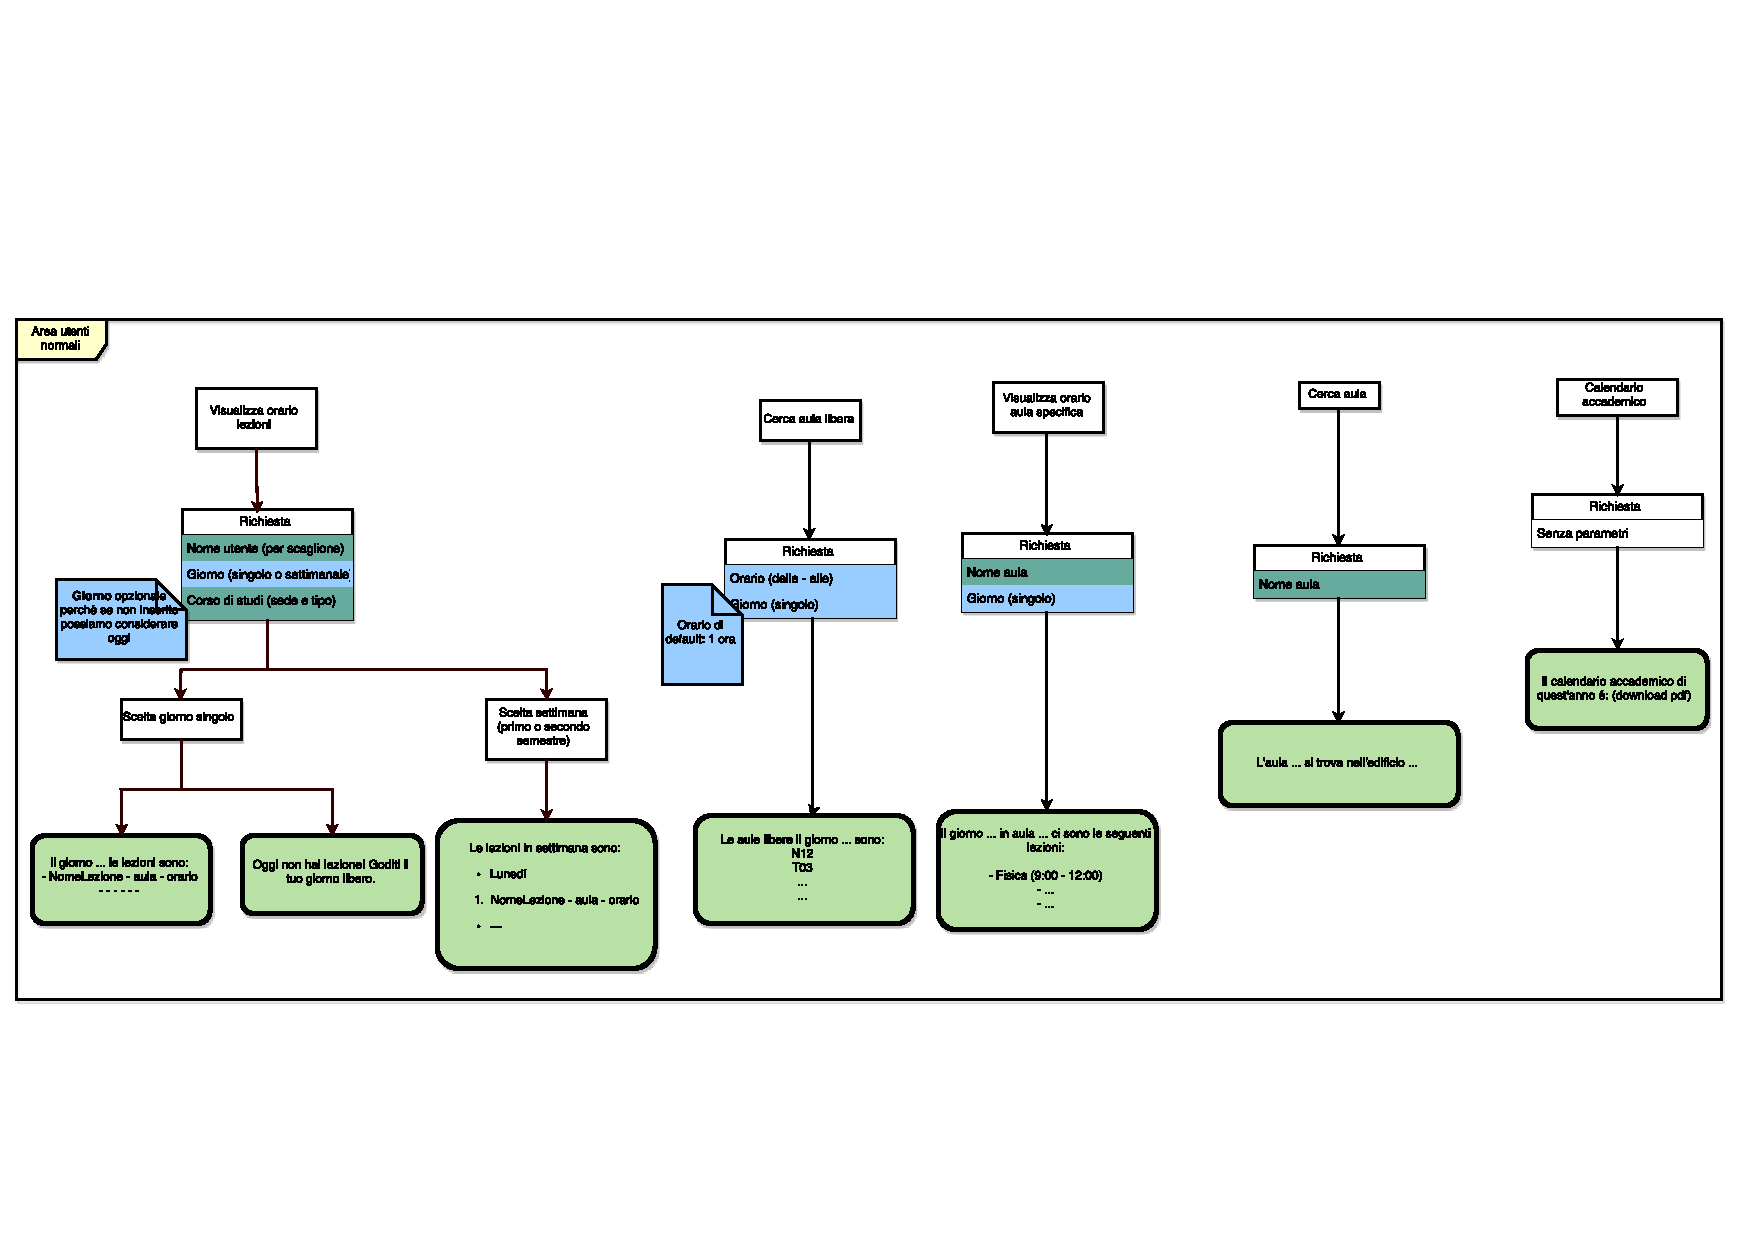
\includegraphics[width=2\textwidth, angle =90 ]{p03}
\thispagestyle{empty}

\vspace*{-3cm}
\hspace*{-3cm} 
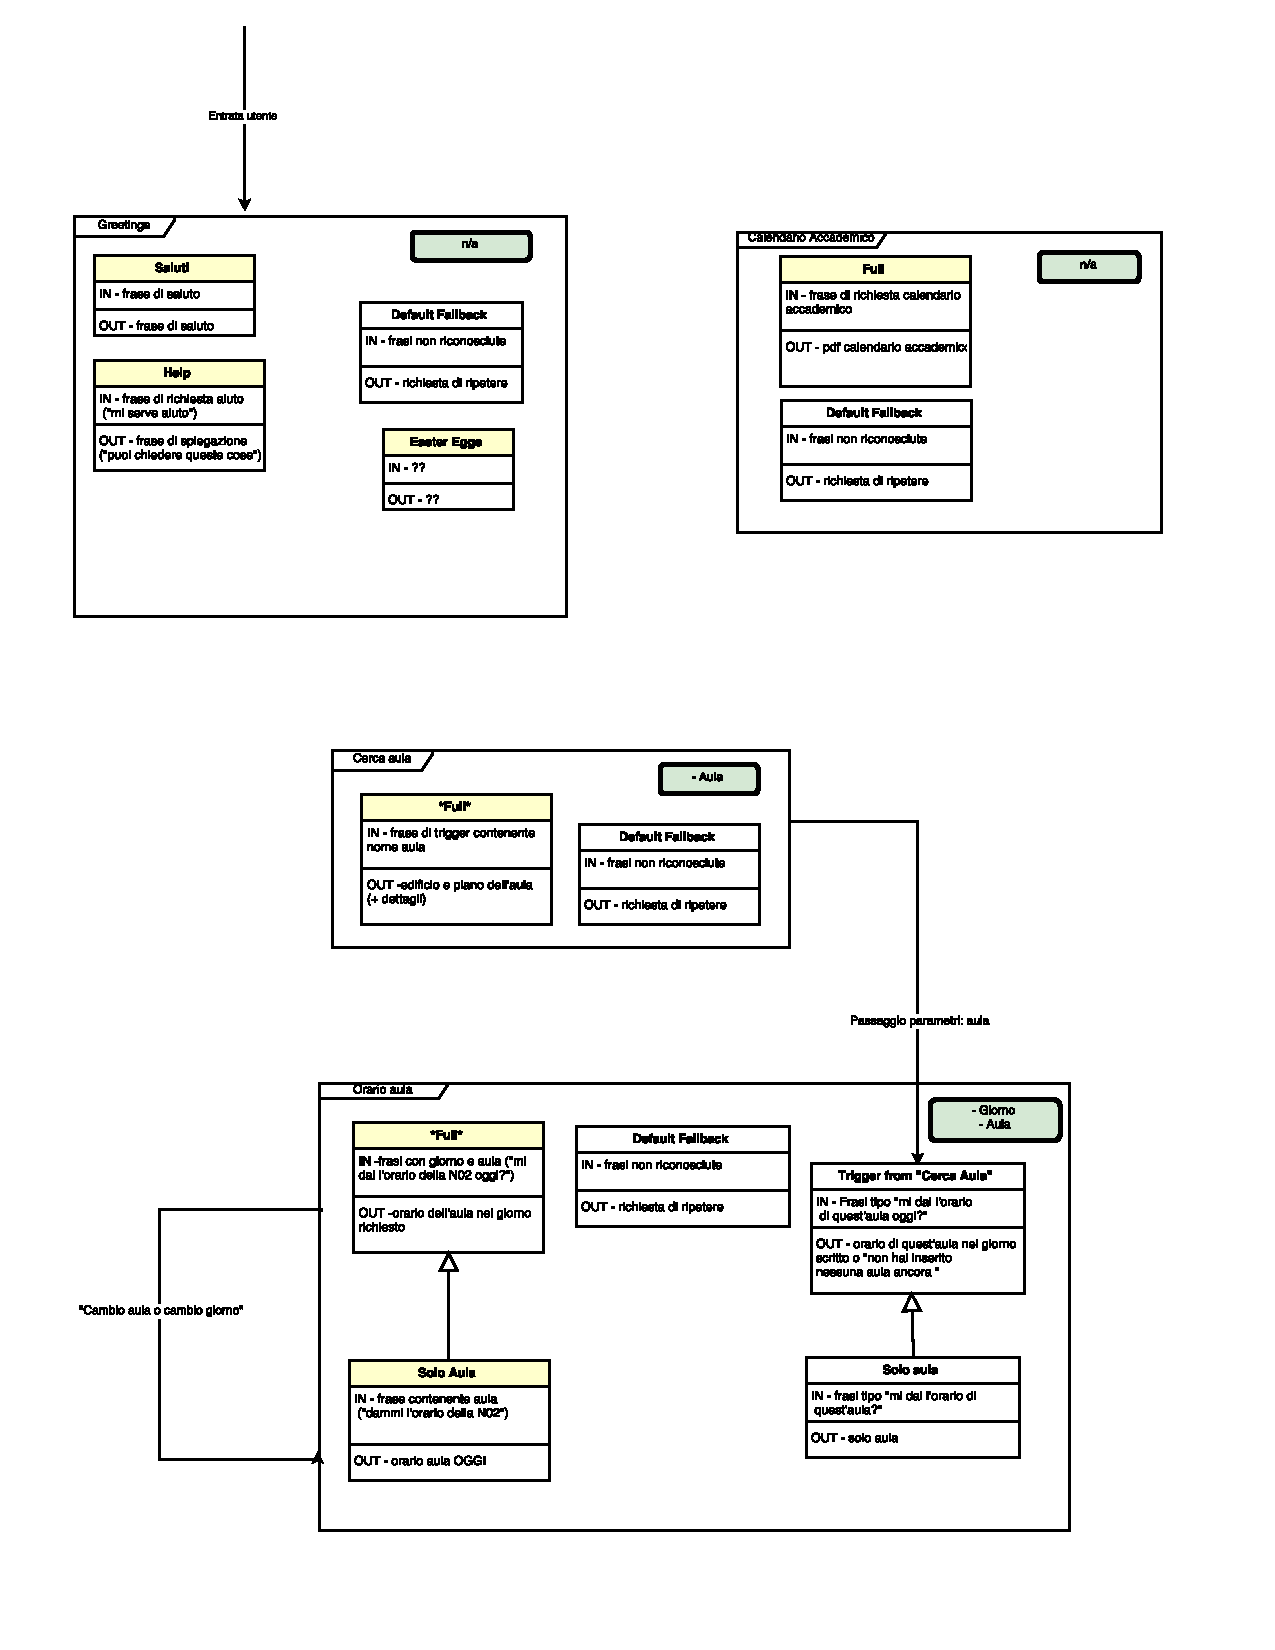
\includegraphics[width=1.6\textwidth]{p05}
\thispagestyle{empty}

\vspace*{-3cm}
\hspace*{-3cm} 
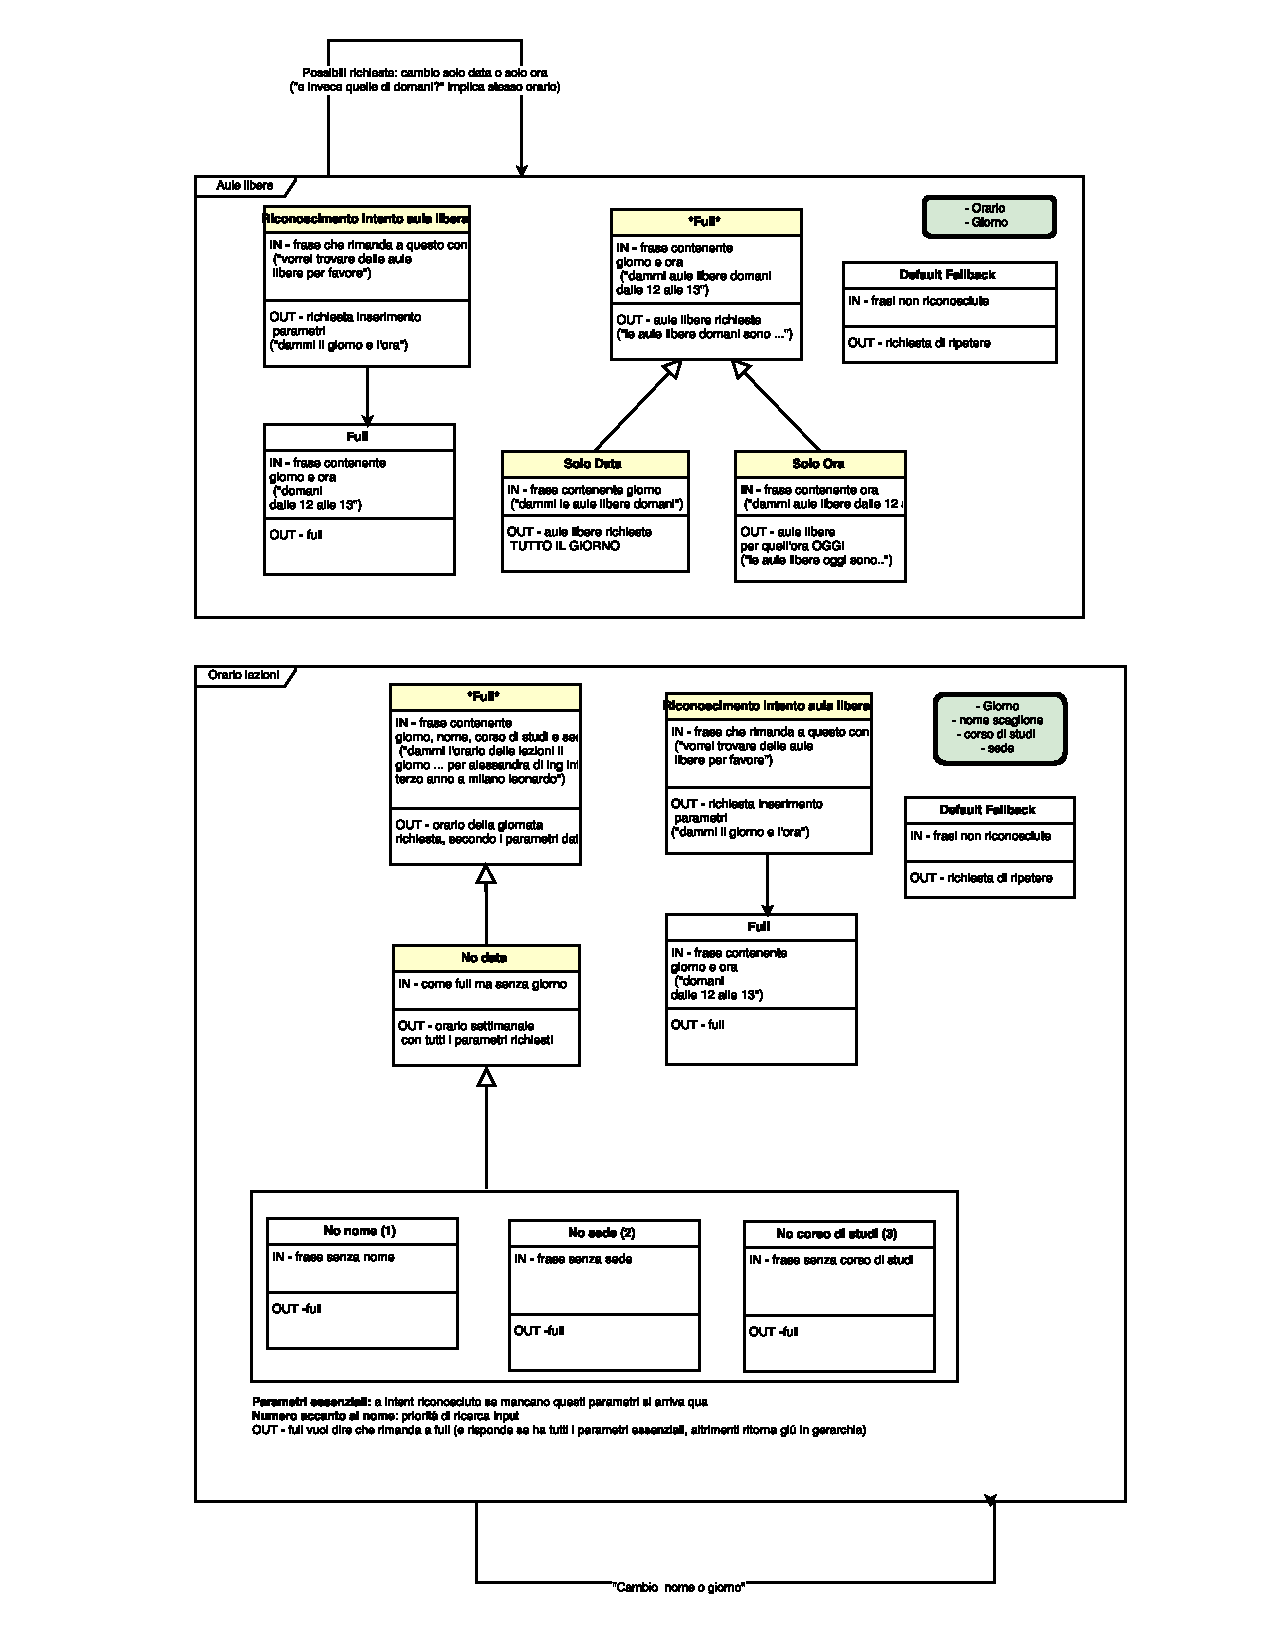
\includegraphics[width=1.6\textwidth]{p04}
\thispagestyle{empty}

\section{Ricerca del FrameWork: Bot di test}
Lo scopo di questa sezione é quello di esplorare il mondo dei framework giá esistenti per trovare la soluzione piú adatta a noi. Pertanto abbiamo pensato che il modo migliore per affrontare il problema sia quello di progettare un chatBot di Test, e implementarlo in ognuna di queste piattaforme. Esso quindi ci aiuterá con la selezione del nostro ambiente di lavoro in base a dei parametri illustrati sotto. É essenziale che sia un bot semplice (per non perdere troppo tempo con lo sviluppo, essendo di test), ma con funzionalitá che siano correlate alla costruzione del nostro progetto in specifica.

\subsection{Requisiti}
\begin{itemize}
\item Interazione basilari con un’API web (bisogna che sia semplice e facile da usare).
\item Riconoscimento domande al bot, piú domande poste in modo diverso devono essere riconosciute (e.g. com'è il tempo domani Milano? = che tempo fa domani a milano?).
\item Riconoscimento semplici entitá date dall’utente (e.g. luogo, ora, data, nome, ..).
\end{itemize}

\subsection{Parametri di valutazione}
Questi rappresentano i parametri che useremo per valutare il framework che testeremo. Essi comprendono sia i componenti di valutazione della costruzione del bot, che quelli piú generali della piattaforma che stiamo usando. La valutazione è a nostra discrezione, ovviamente seguita da una minima descrizione delle procedure svolte.

\paragraph{Bot}
\begin{itemize}
\item \textit{Facilitá di progettazione}: Quante conoscenze e approfondimenti sono necessari per creare il bot.
\item \textit{Tempo di implementazione}: Quanto tempo impieghiamo a creare il bot finito funzionante.
\item \textit{Profondità}: L’insieme di strumenti aggiuntivi che ci sono forniti dall’ambiente di lavoro (training, analisi, ..) che permettono uno sviluppo piú approfondito del bot.
\item \textit{Persistenza della memoria}: possibilitá (e facilitá) di memorizzare certi dati dell’utente per un certo periodo di tempo.
\end{itemize}

\paragraph{FrameWork}
\begin{itemize}
\item \textit{Pricing strategies}: Prezzo e fornitori.
\item \textit{Piattaforme}: Su quali piattaforme di chat (telegram, slack, ..) posso fare il deployment.
\item \textit{Disponibilitá di SDK}: utili allo sviluppo, non enormemente influenti in questo test.
\end{itemize}

\subsection{Descrizione bot}
Il tipo di bot(test) che alla fine abbiamo scelto di portare avanti è una semplice implementazione di chatbot “Che tempo fa?”, cioè data una localitá (milano, monza, ..) e un giorno (oggi, domani, 31/12/2017, ..) restituisce il tempo meteo della localitá scelta nella data scelta. Questo dovrebbe permetterci di esplorare tutti i parametri sopra descritti.
La scelta è ricaduta su questo tipo di bot soprattutto grazie alla disponibilitá di una documentazione passo-passo da parte del frameWork DialogFlow dell'implementazione del bot descritto sopra (presente nella repository di github di riferimento).

\subsection{Deployment description}
In questa parte andiamo a descrivere la nostra esperienza con le 8 (su 25-30 di base) piattaforme individuate tramite un'accurata ricerca. Abbiamo escluso tutte quelle applicazioni per il quale non è stato possibile reperire il prezzo o che proponevano solo dei Trial o Demo (tipicamente pensate per aziende) o quelle che pensiamo non abbiano gli elementi base per poter servire al progetto.
Per l’hosting e il deployment del codice (funzione weatherWebhook) che è servito da base per l’interazione con API esterne, abbiamo usato la piattaforma Google Cloud Project, usufruendo del servizio gratis per 1 anno. Per quanto riguarda l’API key, abbiamo sfruttato quella del famoso sito \url{https://developer.worldweatheronline.com}, che permette di avere la premium key per un periodo di trial di 60 giorni (500 calls per minuto). Una parte su cui abbiamo avuto difficoltá inizialmente è stata la configurazione del servizio di google, ma una volta messo in piedi la struttura della generazione delle risposte dovrebbe essere possibile sfruttare questo script su tutte le piattaforme di testing.

\subsubsection{DialogFlow} 
\paragraph{Implementazione}
La piattaforma permette di creare degli “agent”, contenitori che servono a raccogliere i vari pezzi di riconoscimento delle risposte (“intent”). All’interno di un agent possiamo creare piú intent, cosicché  la struttura finale risultante puó risultare anche abbastanza complessa. Piú intent possono essere concatenati creando un contesto. All’interno di un intent possiamo creare un processo di riconoscimento della domanda data dall’utente, preimpostando una risposta (testuale e non). All’interno del set di domande che l’utente puó scrivere, si possono settare dei “parameter” (gestione quasi automatica del parsing, possiamo comunque scegliere alcuni aspetti del json) che verrebbero quindi usati per la generazione delle risposte. Il riempimento dei parametri puó essere settato per essere preso all’esterno della piattaforma (usando un webHook) in modo molto semplice, inviando e ricevendo sempre un file in formato json. Detto questo è quindi bastato settare un paio di domande e risposte negli intent che abbiamo creato, inserire il giusto indirizzo di webhook e il bot è stato creato e testato su console e sul servizio di chat Telegram.

\begin{center}
\makebox[\textwidth][c]{%
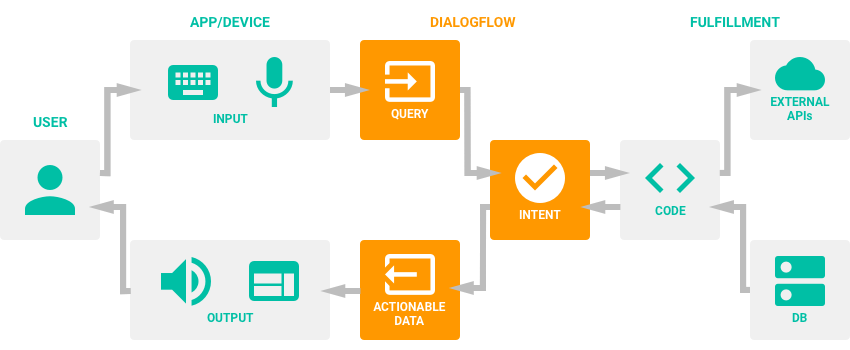
\includegraphics[width=1.2\textwidth]{dialogflow}
}
\footnotesize{Dialogflow in breve}
\end{center}

\paragraph{Valutazione}
\begin{itemize}
\item \textit{Facilitá di progettazione}: \textbf{9} \\ molto semplice e intuitivo, senza bisogno di metter mano a codice

\item \textit{Tempo di implementazione}: \textbf{9} \\ 2 ore (se non contiamo il setting di google cloud)  

\item \textit{Profondità}: \textbf{8} \\  permette di creare facilmente contesti di riconoscimento, presenza di azioni di trigger ed eventi facilmente configurabili, sezione “Training” attivabile, riconoscimente delle domande e parametri non prima specificati
\item \textit{Persistenza della memoria}: \textbf{7} \\ permette di tenere traccia di parametri (settando una lifespan) da poter riusare nel giusto contesto, non abbiamo svolto ulteriori ricerche
\item \textit{Pricing strategies}: \textbf{9} \\ piattaforma completamente gratuita per la progettazione e per il deployment finchè non si raggiungono un certo numero di richieste al minuto, poi hai l’opzione di aumentare il proprio piano

\item \textit{Piattaforme}: \textbf{9} \\ vasta estensione, comprende buona parte dei servizi piú usati ad oggi di chat (messenger, telegram, twitter, ..) e non (slack, google assistant, cortana,..) 
\item \textit{Disponibilitá di SDK}: \textbf{10} \\  presente buona parte dei linguaggi di programmazione piú usati o utili
\end{itemize}

\paragraph{Commento personale}
DialogFlow (ex API.ai) é un ottimo candidato al framework che useremo nel nostro progetto. Semplice e intuitivo, permette di creare semplici o complessi bot se usato nel pieno potenziale, senza perder troppo tempo con il parsing di risposte/domande. Ha molte funzioni interessanti che non abbiamo approfondito, ma che risulterebbero utili al nostro sviluppo. 

\subsubsection{FlowXo}
\paragraph{Implementazione}
FlowXo è il primo servizio nel quale per prima viene chiesta la piattaforma per la quale sviluppare il bot. Ho scelto Telegram: il sito si appoggia a @BotFather per creare e autenticare il proprio bot. Ad un proprio bot è possibile associare un flow, nel quale è possibile assegnare una serie di azioni (tra cui una richiesta http, nel nostro caso).
\paragraph{Valutazione}
\begin{itemize}
\item \textit{Facilitá di progettazione}: \textbf{9} \\ a differenza di altri servizi FlowXo (come suggerisce il nome) focalizza la propria attenzione sul concetto di flow che nel nostro caso è stato piuttosto comodo
\item \textit{Tempo di implementazione}: \textbf{9} \\ 2 ore
\item \textit{Profondità}: \textbf{8} \\ presenta tutte le funzioni base di un servizio del genere
\item \textit{Persistenza della memoria}: \textbf{7} \\ permette di tenere traccia di parametri (settando una lifespan) da poter riusare nel giusto contesto, non abbiamo svolto ulteriori ricerche
\item \textit{Pricing strategies}: \textbf{5} \\ si parte free, per poi passare ad un costo mensile non irrisorio che comprende 5000 interazioni mensili, 15 bot e 3 mesi di log
\item \textit{Piattaforme}: \textbf{4} \\ limitato a Telegram
\item \textit{Disponibilitá di SDK}: n/a
\end{itemize}

\paragraph{Commento personale}
L’utilizzo massiccio del concetto di flow è stato interessante rispetto alle altre soluzioni, ma abbiamo preferito optare per un approccio più libero. Ciò non toglie che tale approccio possa essere più user friendly e intuitivo. Non ci è piaciuto il pricing, avremmo preferito una soluzione free da eventualmente arricchire, piuttosto che un periodo di prova.


\subsubsection{PandoraBots}
PandoraBots offre un servizio di sviluppo di bot molto profondo e personalizzabile. Il tutto è basato su \textbf{AIML (Artificial Intelligent MarkUp Language)}, un’estensione di XML che si è costretti ad imparare se si vuole metter mano a questa piattaforma. Difatti il servizio offerto è quasi solamente dato da interazione con Editor direttamente sul sito. 
\begin{center}
\makebox[\textwidth][c]{%
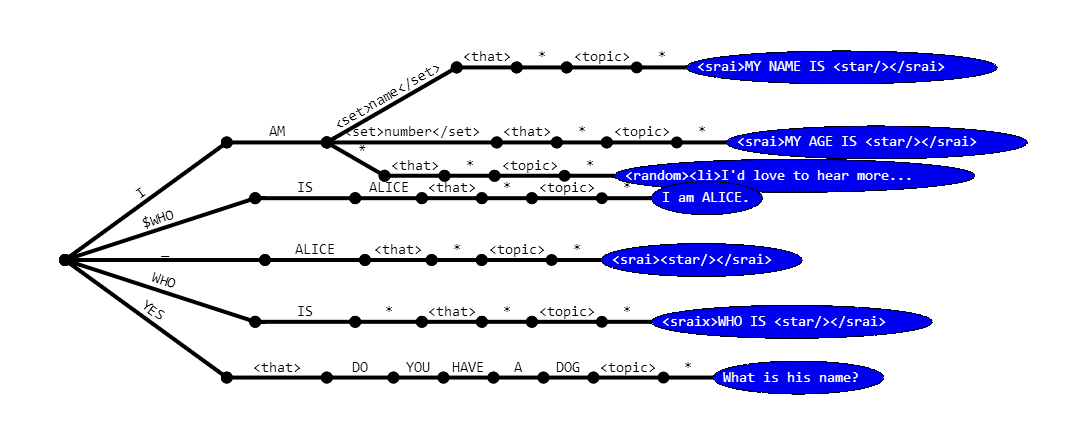
\includegraphics[width=1.2\textwidth]{pandorabots}
}
\footnotesize{AIML Tree view }
\end{center}
\paragraph{Implementazione}
In prima fase è necessario creare un bot e dargli un nome. All’interno possiamo trovare 5 pagine principali, rispettivamente Bot info (modifica informazioni del bot), Train (parlare col bot e cambiare risposte senza entrare in editor), Files (editor di AIML ottimizzato), Log (dove è possibile vedere le singole interazioni col bot) e ClubHouse (possibile pubblicare il proprio bot per farlo parlare con la comunitá). 
Senza andare troppo nel dettaglio con la descrizione del linguaggio AIML (che è stato necessario apprendere), si è dovuto metter mano ai tag in stile XML. <Pattern> (cosa dice l’utente), <Template> (la risposta desiderata a un pattern), <star/> (per “catturare” un input utente) sono solo alcuni dei possibili strumenti che offre questo linguaggio. È possibile creare dei contesti per il quale è possibile richiamare altri template, oppure creare argomenti in cui è possibile “entrare” per dare delle risposte specifiche, appunto in base all’argomento. Il tutto condito dalla possibilitá di aggiungere recursioni o condizioni come un normale linguaggio di programmazione. Queste funzioni base sono servite per creare un semplice bot che riconoscesse localitá e data di una domanda sul tempo, rimandando a un contesto e creando un argomento per chiedere singolarmente data o localitá. Grave mancanza è l’impossibilitá o l’estrema difficoltá di usare del contenuto dinamico, limitato a prendere stringhe da file. 

\paragraph{Valutazione}
\begin{itemize}
\item \textit{Facilitá di progettazione}: \textbf{5} \\ È stato necessario apprendere AIML per poter cominciare a far qualcosa
\item \textit{Tempo di implementazione}: \textbf{7} \\ Una volta apprese le basi di AIML non è stato particolarmente lungo il tempo di sviluppo, 3-4 ore probabilmente
\item \textit{Profondità}: \textbf{8} \\ Al contrario di altre piattaforme, con pandorabots è possibile avere il pieno controllo del proprio bot. Invece scarno per quanto riguarda le funzionalitá accessorie
\item \textit{Persistenza della memoria}: \textbf{10} \\ Grazie alle peculiaritá di AIML è possibile operare come un vero linguaggio, disponendo appunto di costanti e variabili (globali/locali) che si possono manipolare come si vuole
\item \textit{Pricing strategies}: \textbf{8} \\ Lo sviluppo è totalmente gratuito, ma dopo le 1000 interazioni al mese, scatta il tassametro. Possibilitá di esportare il proprio bot localmente e metterlo sul proprio sito
\item \textit{Piattaforme}: \textbf{8} \\ Molte piattaforme supportate come per gli altri frameWork (compreso telegram)
\item \textit{Disponibilitá di SDK}: \textbf{7} \\ Disponibili i soliti Java, Node.js, Python per semplificare l’interazione con l’API di PandoraBots
\end{itemize}
\paragraph{Commento personale}
Di per sé, PandoraBots offre degli strumenti approfonditi per lo sviluppo “dell'intelligenza” sotto al nostro bot, essendo costretti a progettare totalmente da 0 il riconoscimento degli intenti e il flow in generale. La limitazione piú importante è senza dubbio l’impossibilitá di poter sfruttare degli elementi dinamici qualsiasi, o anche solo richiamare API esterne, a noi feature indispensabile. 

\subsubsection{GupShup.io}
\paragraph{Implementazione}
Alla creazione del bot viene chiesto di scegliere innanzitutto se voler manualmente programmare il proprio bot oppure utilizzare un’interfaccia grafica. Nel primo caso si viene reindirizzati ad un IDE, nel quale è possibile partire da zero oppure scegliere un template di partenza e sviluppare quindi su una base già scritta. Nel secondo caso si viene guidati attraverso una GUI piuttosto user friendly, nel quale è possibile sviluppare un bot attraverso un metodo grafico, seppur con funzioni limitate alle basi. Ho ritenuto opportuno testare la prima opzione: qui ho avuto la possibilità di configurare un bot che usasse le funzioni già implementate con DialogFlow con l’utilizzo di un access token. In seguito è stato possibile testare il bot attraverso un proxybot proprietario di GupShup. 

\paragraph{Valutazione}
\begin{itemize}
\item \textit{Facilitá di progettazione}: \textbf{8} \\ è opportuno sottolineare che il sito offre due esperienze di progettazione completamente opposte: da un lato viene data completa gestione allo sviluppatore, con conseguenti maggiori opzioni, mentre dall’altro viene offerta un’esperienza radicalmente più semplice ma comunque efficace per bot meno complessi.
\item \textit{Tempo di implementazione}: \textbf{9} \\ il giudizio è chiaramente riferito all’opzione grafica, mentre non è possibile dare un giudizio in merito allo sviluppo effettivo usando la prima opzione
\item \textit{Profondità}: \textbf{7} \\  le due opzioni offrono profondità diametralmente opposte: l’uso dell’IDE permette di avere una completa libertà, mentre l’uso dell’opzione grafica è incredibilmente limitante (sebbene sia effettivamente consigliato solo per uno sviluppo di base)
\item \textit{Persistenza della memoria}: \textbf{6} \\ avendo testato attraverso il bot di DialogFlow il giudizio è il medesimo
\item \textit{Pricing strategies}: \textbf{8} \\  piattaforma completamente gratuita e senza vincoli di progettazione, possibilitá di richiedere informazione di prezzo personalizzate a seconda delle interazioni (business type)
\item \textit{Piattaforme}: \textbf{9} \\ comprende pressoché tutte le piattaforme più diffuse
\item \textit{Disponibilitá di SDK}: \textbf{7} \\ l’IDE permette di usare JavaScript e Node.js
\end{itemize}

\paragraph{Commento personale}
Il servizio è ottimo ed è utile sia all’utente più navigato sia ad un utente meno esperto. L’integrazione con DialogFlow è assolutamente di centrale importanza, permettendo ad un bot sviluppato con tale servizio di essere implementato senza problemi anche su GupShup.


\subsubsection{Microsoft Bot Framework}
Il frameWork di windows comprende molti strumenti, ma ci offre un’esperienza troppo macchinosa e non prettamente indirizzata alla progettazione del chatBot come le altre piattaforme. Prima di tutto occorre sottolineare che l’applicazione offre 3 servizi principali:
\begin{enumerate}
\item Azure Bot Service - fornisce le risorse necessarie per l’hosting (a pagamento), il deployment e l’editing del bot (tramite editor o interfacciandosi a IDE tipo VisualStudio)
\item Bot Builder - insieme di SDK utili alla costruzione del bot. Nativamente supporta C\# e Node.js, mentre si ha la possibilitá di usare tutti gli altri tipi di linguaggi tramite una REST api
\item Bot FrameWork Portal - portale principale di accesso al Framework, permette la manipolazione delle informazioni di base del bot, la creazione di nuovi e prevede una piattaforma di testing
\end{enumerate}
La costruzione di un bot all’interno di Microsoft Bot Framework avviene solo ed esclusivamente tramite programmazione “vecchia maniera”, ovvero tramite progettazione su carta e sviluppo con un linguaggio di programmazione a piacere, gestendo le domande e il flow delle risposte a piacimento. Non c’è ovviamente nessun Intent Recognition di base, a meno che non si usino delle chiamate di API  NLU (LUIS di Microsoft - a pagamento ovviamente - o esterne). Grazie alla possibilitá di poter sviluppare con righe di codice il proprio bot è ovviamente favorita la personalizzazione e il controllo. È presente inoltre un connector service che collega il codice con qualsiasi tipo di applicazione input/output vogliamo. Sono ovviamente presenti degli strumenti di test e debug indirizzati in particolare a questo argomento. Nota molto positiva è la ricca documentazione, anche perché nella sezione di design del bot è presente la formalizzazione di alcuni concetti molto significativi nello studio dell’efficacia di un bot.
\begin{center}
\makebox[\textwidth][c]{%
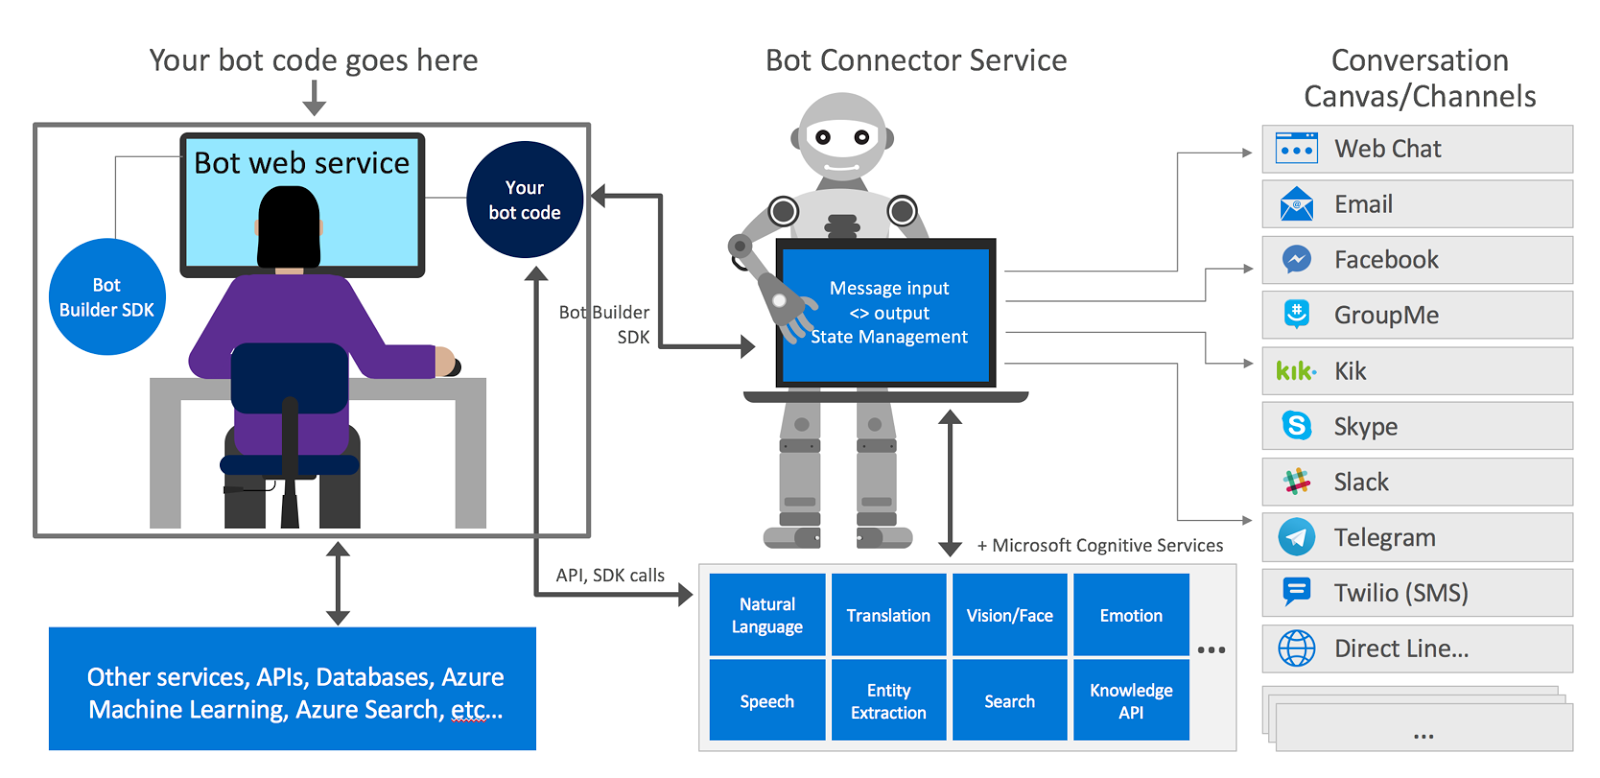
\includegraphics[width=1.2\textwidth]{mbf}
}
\footnotesize{Microsoft Bot FrameWork overview}
\end{center}
\paragraph{Conclusioni}
 Ci è stato chiesto di “esplorare” il neonato mondo dei bot, in particolare ChatBot alla ricerca della migliore alternativa (in base a parametri di personale importanza) di sviluppo dello stesso. Pur essendo informatici, non avendo paura della possibilitá di tuffarsi sull’apprendimento di un linguaggio di programmazione a noi non noto e apprezzando il poter avere la libertá di scrivere codice, consideriamo questo approccio poco adatto al nostro progetto in quanto “”obsoleto”” e poco innovativo, oltre a portarci via potenzialmente troppo tempo.
 
\subsubsection{Wit.ai}
Dopo aver consultato la guida per iniziare e aver cominciato a creare qualcosa, mi son reso conto che mancavano delle funzioni significative. Ho appreso che facebook sta chiudendo la piattaforma in modo da integrare il “natural language processing (NPL)  tools into Messenger Platform 2.1”

\subsubsection{ChatFuel}
\paragraph{Implementazione}
Nel servizio è presente solo la possibilitá di maneggiare la struttura del bot solo tramite GUI. Interfaccia molto semplice, presenza di “Blocks” che permettono di modellare l’automatizzazione di azioni (presa input, richieste http, stampa video,..) e “Groups” nella quale racchiudere a piacimento questi blocks. I suddetti blocchi possono essere concatenati in sequenze a seconda del bisogno, ed esistono strutture che permettono di maneggiare queste transizioni (da blocco a blocco - da sequenza a sequenza) in modo quasi intuitivo e completo. Questi blocchi possono avere una vasta gamma di eventi di trigger, ma principalmente vengono richiamati dalla sezione ”””””AI””””” che permette di inserire delle frasi (con “riconoscimento del contesto”)  ed eseguire di conseguenza un dato blocco. Dopo aver capito i funzionamenti base della piattaforma dunque è bastato creare un singolo blocco con la giusta presa di input dall’utente e una richiesta http per creare il bot desiderato. Da notare l’impossibilitá di testare il bot su una qualche console ma solo direttamente sulla propria pagina facebook (alla quale si deve per forza collegare il bot). Per completezza del documento, in questa piattaforma è stato necessario ri-adattare il codice in Node.js descritto all’inizio di questo testo, in modo che ricevesse del codice Json in entrata e uscita leggermente diversi, come scritto sulla repository di github.

\begin{center}
\makebox[\textwidth][c]{%
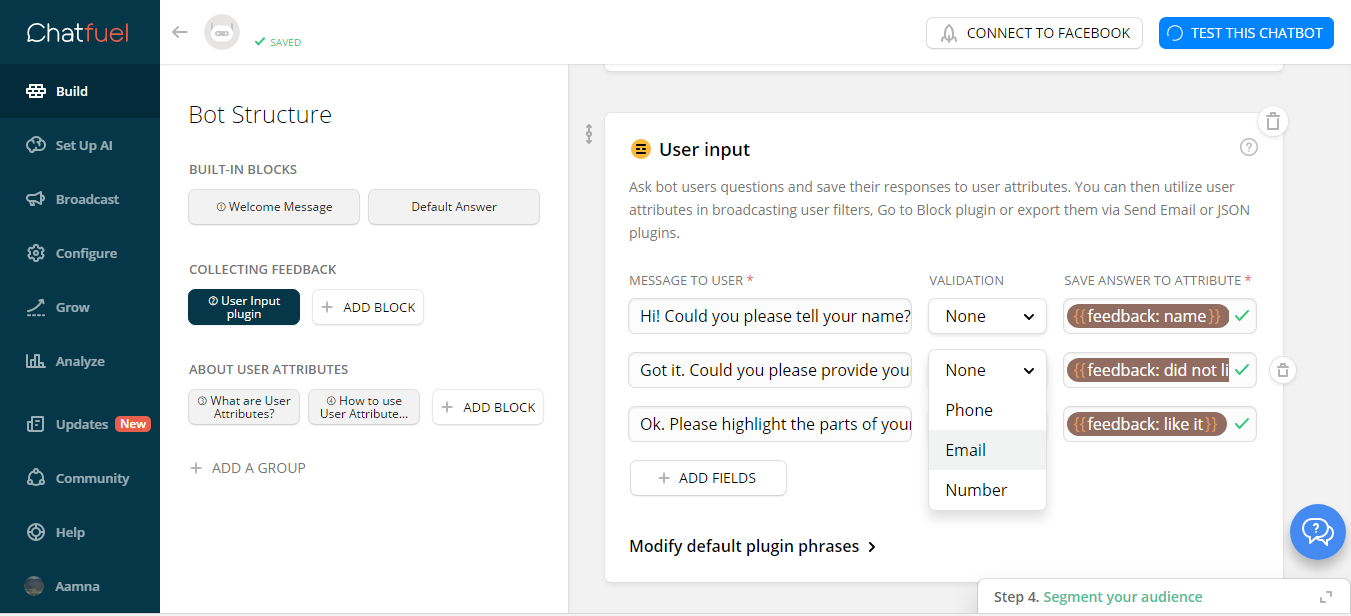
\includegraphics[width=1.2\textwidth]{chatfuel}
}
\footnotesize{Panoramica della piattaforma (user input plugin)}
\end{center}

\paragraph{Valutazione}
\begin{itemize}
\item \textit{Facilitá di progettazione}: \textbf{8} \\ A parte la difficoltá nel trovare il giusto formato Json, l’intera piattaforma è molto intuitiva (presente solo interfaccia grafica)
\item \textit{Tempo di implementazione}: \textbf{9} \\ 2,5 ore, senza contare lo sviluppo del motore su Google Cloud (giá fatto per altri framework)
\item \textit{Profondità}: \textbf{6} \\ Da un lato è molto limitante (ad esempio, non è possibile fare un parsing di una frase in modo da ottenere specifici parametri, ma si deve dar la possibilitá all’utente di inserirli volta per volta), dall’altro è interessante la possibilitá di usare Plugin modulabili a piacimento (sia interni che esterni), anche se preimpostati. Presenza di diversi tool di analisi e broadcast facile
\item \textit{Persistenza della memoria}: \textbf{6} \\  All’interno di un blocco è possibile tenere traccia delle variabili o parametri dell’utente
\item \textit{Pricing strategies}: \textbf{8} \\  piattaforma gratuita, ma previa creazione di pagina facebook. Possibilitá di sottoscrivere abbonamento per un servizio migliore
\item \textit{Piattaforme}: \textbf{3} \\ Implementato solo in facebook
\item \textit{Disponibilitá di SDK}: \textbf{9} \\ n/a
\end{itemize}
\paragraph{Commento personale}
Con questo framework non è possibile creare bot troppo sofisticati, in quanto non sono possibili certe azioni come il riconoscimento automatico di parametri in una frase complessa data dall’utente. È invece, a mio parere, molto consigliato per chi deve gestire una pagina facebook con chat automatica del tipo “botta e risposta”. Fornisci i comandi e l’applicazione esegue delle azioni. Stop. Carina la presenza (anche se non richiesta come requisito nelle nostre specifiche) dell’integrazione di vari tool di analisi della crescita e popolaritá, come giustamente mi aspetto da una piattaforma sviluppata unicamente per un social network.


\subsubsection{kitt.ai}
\paragraph{Implementazione} 
Dopo un’accurata lettura dei docs di riferimento, è stato possibile iniziare a sviluppare il bot di test. Per prima cosa si è dovuto aggiungere alla workZone i nodi di ChatIn e ChatOut (per impostare l’inizio e fine del flow), successivamente in mezzo a essi il nodo router (un piú o meno semplice if condizionato, collegato a ogni enter node (condizioni di entrata del ramo) che permette la scelta del ramo nei vari casi di funzionamento. Questi casi possono essere piú o meno complessi. Per il parsing della frase d’entrata data dall’utente è stato necessario creare un semplice riconoscimento d’intenti con la piattaforma per NLU (natural language understanding) direttamente da kitt.ai (anche se è possibile collegare diverse NLU, tra cui anche dialogflow). Una volta che sono stati fatti i vari rami di condizione, è bastato aggiungere le varie risposte e un minimo di codice per costruire il Json da passare alla nostra richiesta http. Per questa richiesta è possibile aggiungere un nodo http request che, settando alcuni parametri fondamentali, non ha avuto problemi a consegnarci la risposta che aspettavamo dalla funzione attiva su google cloud. Questa volta è stato necessario modificare leggermente l’output del cloud poiché era scomodo inviare un Json, comodo invece una semplice stringa. 

\begin{center}
\makebox[\textwidth][c]{%
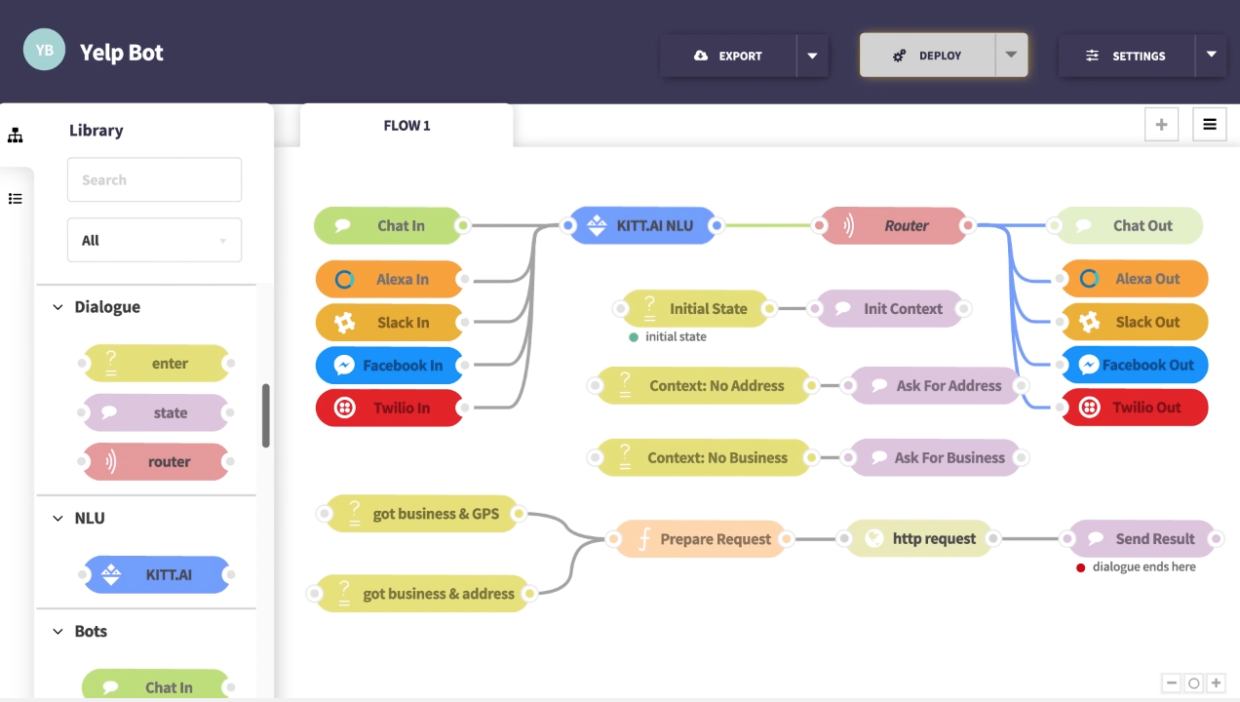
\includegraphics[width=1.2\textwidth]{kittai}
}
\footnotesize{kitt.ai GUI overview}
\end{center}

\paragraph{Valutazione} 
\begin{itemize}
\item \textit{Facilitá di progettazione}: \textbf{8} \\ Dopo una lettura delle docs (piú che altro per capire i vari formati dei messaggi e il funzionamento dei nodi) non è stato assolutamente difficile crearlo. Molto bella e funzionale la GUI, che ti permette di avere una visione chiara del flow del codice
\item \textit{Tempo di implementazione}: \textbf{8} \\ 3 ore, la maggior parte speso per varie prove e test
\item \textit{Profondità}: \textbf{9} \\ possibile programmazione in javascript direttamente nel flusso tramite alcuni nodi, integrazione nativa di alcune API e possibilitá di aggiungere le tue, comodo debug da programmare come vuoi e vasta gamma di nodi funzione per poter creare quello che vuoi
\item \textit{Persistenza della memoria}: \textbf{10} \\ Ho trovato molto semplice e comodo “giocare” con le variabili globali o locali (del messaggio ricevuto). La docs è molto dettagliata su come usare e creare le varie entitá
\item \textit{Pricing strategies}: \textbf{8} \\ Il framework è in fase beta, ma è possibile richiedere e ricevere una key apposta. Gratis fino a un certo numero di interrogazioni, poi richiesta il passaggio a un piano a pagamento
\item \textit{Piattaforme}: \textbf{10} \\  la maggior parte delle piattaforme Business e Private sono supportate
\item \textit{Disponibilitá di SDK}: n/a
\end{itemize}
\paragraph{Commento personale}
Nell’insieme questo framework mi sembra un buon candidato alla fase finale del nostro progetto, poiché concilia facilitá di utilizzo con possibilitá abbastanza profonda di personalizzazione. Bisogna vedere come si comporta con applicazioni piú grandi. Purtroppo è ancora in fase beta, quindi il suo futuro è abbastanza incerto, ma è stato comunque interessante poter apprendere una logica diversa su cui è stato possibile approfondire il concetto di ChatBot.


\subsection{Commenti Finali e decisione}
Non c'é molto da dire, il framework che ci ha convinto di piú é \textbf{DialogFlow}, che unisce alla semplicitá e intuitivitá di sviluppo del bot a una grande profonditá di azioni che é possibile compiere, senza rinunciare a svariati tool di apprendimento e gestione che a noi sono risultati comodi. Note di merito vanno comunque a PandoraBots, che permette di costruirsi il proprio riconoscimento d'intenti, e kitt.ai, che utilizza la migliore interfaccia tra tutti i sopracitati ambienti. 

\section{Costruzione bot di Demo}
Dopo aver quindi svolto un lungo lavoro di ricerca abbiamo le conoscenze necessarie per costruire la demo del bot. Appunto perchè si tratta di una prova optiamo per una versione "limitata" del progetto, che però ci permette di utilizzare e consolidare le conosceze acquisite nella parte precedente. Tutte le limitazioni rispetto all'idea originale sono presenti nella sezione apposita, mentre nelle prime due sono descritti in linea di massima le principali componenti e le nostre soluzioni di implementazione. Avendo ben definito queste due parti, ci è venuto naturale dividerci i compiti tra chi si sarebbe occupato di scrivere il codice nella parte server (Stefano) e chi si sarebbe invece dedicato alla struttura della conversazione (Paolo).

\subsection{ServerSide}
A livello server abbiamo ritenuto opportuno seguire lo stesso procedimento adottato per il test delle piattaforme, ovvero impostare un webhook. A differenza del test con l’API di  \url{https://developer.worldweatheronline.com} abbiamo dovuto scrivere del codice Javascript adatto a gestire le richieste del nostro PolimiBot. Per impostare il webhook per tale scopo abbiamo deciso di utilizzare i servizi offerti dalla piattaforma Google Cloud Platform e utilizzare una Cloud Function con il codice Javascript sopra citato. 
Il principio di base è eseguire una specifica funzione a seconda della richiesta dell’utente: più nello specifico abbiamo deciso di utilizzare uno switch basato sul contesto inviato all’interno del JSON del richiedente. Inizialmente si era pensato di usare uno switch sugli intenti: tale approccio è risultato non adatto poiché non permetteva di gestire multiple richieste consecutive nel medesimo contesto. (es. chiedere la posizione di più aule consecutivamente) 
La gestione dei dati degli eventuali utenti è stata una scelta più difficile: dapprima abbiamo provato ad utilizzare il servizio di Cloud SQL (sempre offerto da Google Cloud Platform), ma non avendo dimestichezza con i database abbiamo deciso di non seguire questa idea. Abbiamo quindi ragionato sui corsi di studio e sulle competenze acquisite e abbiamo deciso di utilizzare dei file JSON come già praticato durante il corso di Ingegneria del Software: oltre alla motivazione sopra descritta è opportuno sottolineare che il frontend comunica con il backend utilizzando dei JSON, quindi ci è sembrato naturale scegliere quel formato.
L’uso dei file JSON ci ha permesso non solo di gestirle multiple sorgenti di dati, ma anche di avere librerie già adibite alla lettura e alla manipolazione dei file JSON: tali file possono inoltre essere scorporati dal codice e usati in un server locale, qualora ce ne fosse la necessità.

\subsection{UX (DialogFlow)}
La parte in cui viene modellata la conversazione macchina-utente è interamente contenuta in DialogFlow. In buona parte la piattaforma è descritta nella sezione dedicata alla scelta del framework. Si è cercato di seguire il più fedelmente possibile lo schema descritto sopra di interazione tra i contesti. Usando DialogFlow non ho avuto molta difficoltà a creare le relazioni tra intenti che cercavamo, più difficile invece è stato creare i contesti e utilizzarli in modo efficace (con il passaggio di parametri sopra descritto nel passaggio tra contesti). Il riconoscimento di parametri è molto valido se si tratta di parametri di sistema (e.g.\ data, ora, period), mentre è stato necessario crearne di personali per aule e corsi di studi. Questa ultima parte è abbastanza noiosa in quanto, per avere la maggior accuratezza possibile, dovresti inserire tutti i possibili valori con i relativi sinonimi (a meno che non voglia rischiare di riconoscere parametri non corretti). Tutto sommato però, dopo aver passato qualche ora a ragionare sulle diverse relazioni tra contesti e intenti, è venuto fuori un bot completo, come appunto descritto nello schema a oggetti.  

\subsection{Limitazioni}
Ecco i principali punti che descrivono in cosa questa demo si discosta dal progetto completo:
\begin{itemize}
\item Motore di Scraping costruito "ad-Hoc" (informazioni non dinamiche), cioè posto come formato json come costante all'interno del codice sul server.
\item Implementata solo parte utenti NON loggati.
\item Persistenza assente.
\item  Non completata la parte server di orari lezioni, implementata solo su dialogflow.
\end{itemize}

\section{Futuri Sviluppi}
Cosa ci aspetta il futuro? Ecco cosa ci piacerebbe implementare e come intenderemmo farlo:
\begin{itemize}
\item Completare la parte degli utenti non loggati con tutte le sue parti funzionanti nel codice server.
\item utilizzare uno scraping che permetta di manipolare informazioni dinamiche: può essere comunque utilizzato un motore che "crei" un json in modo da non dover cambiare la struttura del nostro codice, o perlomeno apportare solo piccole modifiche.
\item trovare la migliore soluzione per quanto riguarda la memorizzazione dei dati. Si pensava inizialmente di mettere tutto dentro un file di testo sotto una voce univoca che rappresenta l'utente.
\item implementare il riconoscimento utente tramite controllo codice univoco della piattaforma (dialogflow in questo caso). A seconda delle informazioni che troviamo l'esperienza verrà personalizzata.
\item cercare soluzioni per ottenere un livello di pivacy accettabile in modo da poter richiedere informazioni delicate quali codice persona e password.
\item trovare un modo efficace per utilizzare queste informazioni tramite il motore di scraping sopra citato. Ovviamente devono essere utilizzate in modo da mantenere il livello di privacy minimo richiesto.
\item implementare quindi tutte le funzionalitá utente loggato, meno gli avvisi personalizzati.
\item costruire evento trigger invio notifica, parte che richiede uno studio piú approfondito.
\end{itemize}

\newpage

\begin{thebibliography}{9}
\bibitem{dialogflow} 
\textbf{DialogFlow}: \url{https://dialogflow.com}
 
\bibitem{gitHub} 
\textbf{Repository GitHub}: \url{https://github.com/Roncax/PolimiChatBot}
 
\bibitem{google cloud} 
\textbf{Google Cloud Platform}: \url{https://cloud.google.com}
 
\bibitem{microsoft article} 
Utile articolo di design principles: \url{https://docs.microsoft.com/en-us/bot-framework/bot-service-design-principles}

\bibitem{google docs} 
Google DialogFlow docs: \url{https://dialogflow.com/docs/getting-started/basics}

\bibitem{designarticle}
Altro utile articolo sul design di un chatbot: \url{https://chatbotsmagazine.com/design-framework-for-chatbots-aa27060c4ea3}

\end{thebibliography}




\end{document}
